\documentclass[conference]{IEEEtran}

\usepackage[utf8]{inputenc}
\usepackage[T1]{fontenc}
\usepackage{amsmath}
\usepackage{graphicx}
\usepackage{booktabs}
\usepackage{array}
\usepackage{tikz}
\usetikzlibrary{positioning,arrows.meta,fit,calc}
\usepackage{pgfplots}
\pgfplotsset{compat=1.17}
\usepackage{balance}
\usepackage{xurl}
\usepackage[hidelinks]{hyperref}

\begin{document}

\title{Avalux: An Open Integrated Platform for Moderated Usability Testing
with Real-Time Evaluator--Participant Synchronization}

\author{\IEEEauthorblockN{Hugo Correia, Bernardo Marques, and Samuel Silva}
\IEEEauthorblockA{IEETA / DETI, University of Aveiro\\
Aveiro, Portugal\\
\{hf.correia, bernardo.marques, sss\}@ua.pt}}

\maketitle

\begin{abstract}
Moderated usability testing remains the reference method for discovering
interaction problems, yet its instrumentation is fragmented: evaluators
juggle stopwatches, spreadsheets, questionnaire tools, and manual report
assembly, while commercial platforms focus on unmoderated remote studies
whose moderated modes capture video and free-form notes rather than
structured per-task metrics. We present
Avalux, an open, self-hostable web platform that integrates the complete
moderated-testing pipeline: reusable test protocols (tasks with optimal-path
baselines, typed error taxonomies, per-task questions including in-browser
audio/video/photo capture, interview scripts, and study-specific participant
attributes); a live evaluator cockpit that logs per-task completion time,
action counts, categorized errors, hesitation events, and Single Ease
Question ratings; and a participant client that runs on the participant's
own device via a join link, synchronized with the evaluator in real time
over WebSocket channels, including a gating protocol that prevents the
session from advancing while the participant is still answering. Sessions
can conclude with a semi-structured interview and with whichever
automatically scored questionnaires a study selects, among them the System
Usability Scale, and export to a self-contained PDF report.
For teaching, a further layer turns properties of the methods into figures
students compute on their own work: independent heuristic inspection that
reports how far evaluators agreed, a comparison of inspection predictions
with what participants actually encountered, reflection after each session
drawn from what the session recorded, a kept record of every protocol
revision, and a class-wide view for the instructor.
We describe the architecture, a React single-page application over a
Postgres backend with row-level security, and report two case studies:
a four-participant evaluation of a household touch-panel controller
(mean SUS 28.1) and a two-participant evaluation of an eye-tracking
analysis dashboard (SUS 80). The studies show that the platform
carries complete, realistic evaluations end to end, including a physical
device beyond the reach of browser-based instrumentation, while
producing diagnostic task-level detail alongside the standard summary
metrics.
\end{abstract}

\begin{IEEEkeywords}
usability testing, moderated evaluation, heuristic evaluation, SUS, SEQ,
HCI education, research tools, human--computer interaction
\end{IEEEkeywords}

\section{Introduction}
Task-based moderated testing with a small number of participants remains
the workhorse of usability practice: a facilitator observes a participant
attempting representative tasks, records performance and difficulties, and
complements observation with standardized instruments such as the System
Usability Scale (SUS)~\cite{brooke1996sus} and the Single Ease Question
(SEQ)~\cite{sauro2009comparison}. Classic problem-discovery models show
that even four to five participants uncover the majority of severe
problems~\cite{virzi1992refining,nielsen1993mathematical}, which keeps the
method attractive for small teams and academic projects.

The tooling situation is less attractive. Commercial platforms concentrate
on unmoderated remote studies, where metrics are captured by automatic
instrumentation of the participant's browser; their moderated modes
produce session videos and free-form notes that must be coded after the
fact. In practice, a moderated session is therefore run with an ad-hoc
toolchain (a stopwatch, a paper or spreadsheet observation grid, a
separate questionnaire form, and manual report writing) that is slow,
error-prone, and hard to standardize across studies. The cost is not only
effort: a measurement in that toolchain is written down three times, once
while observing, once when it is transferred for analysis, and once when it
reaches the report, and no copy is authoritative.
Section~\ref{sec:integration} argues what integration buys in exchange, and
what it costs.

This paper presents \emph{Avalux}, an open web platform that integrates
the moderated-testing pipeline end to end. Its contributions are:
\begin{itemize}
  \item an \textbf{integrated protocol model}: reusable templates couple
  tasks (with optimal time and action-count baselines) to typed error
  taxonomies, per-task questions (open, choice, rating, and in-browser
  audio/video/photo capture), interview scripts, and study-specific
  participant attributes;
  \item a \textbf{live moderated session} design in which the evaluator's
  cockpit (timer, action counter, one-tap typed error and hesitation
  logging, per-task SEQ) and the participant's own device are synchronized
  in real time, including a gating protocol that blocks task advancement
  while the participant is still answering the previous task's questions;
  \item \textbf{two case studies}, a household touch-panel controller and
  an eye-tracking analysis dashboard, both run entirely on the platform,
  showing that it carries realistic studies end to end, including a
  physical device beyond browser instrumentation, and that its task-level
  instruments localize the problems behind widely differing outcomes
  (mean SUS 28.1 vs.\ 80);
  \item a \textbf{pedagogical design} for classroom use, mapped onto
  empirically reported learning difficulties, in which features are chosen
  for the evidence they produce about the method rather than for the effort
  they save: independent heuristic inspection with an agreement statistic,
  a comparison of inspection predictions against observed problems,
  co-rating, evidence-grounded reflection, a protocol review and an optional
  instructor gate with a kept revision history, and a class view for the
  instructor.
\end{itemize}

Avalux is deployed at \url{https://avalux.pt}; its schema, protocol
seeds, and report generator are versioned with the application source.

\section{Related Work}

A mature market of commercial software-as-a-service platforms now supports remote usability evaluation. UserTesting combines a proprietary participant panel with video-first moderated (``Live Conversation'') and unmoderated studies overlaid with AI-assisted analysis~\cite{usertesting2026platform}, and has absorbed the quantitative benchmarking platform UserZoom following their 2023 merger~\cite{usertesting2026userzoom}. Maze is unmoderated by default, converting prototypes and live websites into task-based studies scored through automatically instrumented metrics such as completion rate, misclick rate, and task duration~\cite{maze2026platform}. Lookback specializes in live moderated sessions with screen, camera, and audio capture, stakeholder observation rooms, and timestamped free-form notes~\cite{lookback2026platform}; Loop11 supports both modes and, unusually, auto-computes SUS and NPS for unmoderated tests~\cite{loop112026platform}; Useberry targets prototype-centric unmoderated testing with click and flow analytics~\cite{useberry2026platform}. Across these tools, quantitative evidence derives almost entirely from automated client-side instrumentation in unmoderated studies, while moderated modes yield video recordings and free-form notes that must be coded after the fact. To the best of our knowledge, none \emph{combines} structured real-time evaluator logging in moderated sessions, per-task ease ratings integrated into the same pipeline, and an open, self-hostable architecture in one platform.

Academic work on remote evaluation dates to Hartson et al., who framed the network as an extension of the usability laboratory~\cite{hartson1996remote}. Andreasen et al.\ subsequently found remote synchronous testing ``virtually equivalent'' to conventional lab-based think-aloud, whereas asynchronous methods identify fewer problems at lower moderator cost~\cite{andreasen2007remote}, an asymmetry confirmed by Bruun et al.~\cite{bruun2009asynchronous} and persisting in recent comparisons~\cite{alhadreti2022comparison}. On the tooling side, RemUSINE and WebRemUSINE pioneered task-level instrumentation by comparing interaction logs against task models, but operate post hoc rather than steering live sessions~\cite{paterno2000remusine,paganelli2003webremusine}. TechSmith's Morae became the de facto observation suite in usability practice~\cite{techsmith2004morae,bastien2010usability}; its Observer component supported real-time marker and error logging by observers during moderated sessions and is the closest precedent to our evaluator instrument, but Morae is a discontinued desktop product requiring installed software on the participant's machine, without participant-side questioning or an open architecture. More recent browser-based platforms such as UTAssistant~\cite{desolda2017utassistant,federici2018utassistant} and the analytics-augmented test-management system of Generosi et al.~\cite{generosi2022test} target largely asynchronous workflows, and an action-research deployment of remote testing found the evaluation tool itself to be an obstacle to high-quality results~\cite{pedersen2021asynchronous}.

Avalux's measurement model follows the ISO 9241-11 decomposition of usability into effectiveness, efficiency, and satisfaction~\cite{iso2018usability}. Perceived usability is captured with the ten-item SUS~\cite{brooke1996sus}, whose reliability~\cite{bangor2008empirical,lewis2018sus}, benchmark mean of 68~\cite{sauro2011practical}, and adjective-based interpretation~\cite{bangor2009determining} are well established; per-task difficulty uses the Single Ease Question, shown to perform comparably to more elaborate post-task instruments~\cite{sauro2009comparison}. Completion rate, time-on-task, and action counts relative to an optimal path are the standard objective performance metrics~\cite{albert2022measuring,sauro2016quantifying}, and moderated testing with small samples is supported by classic problem-discovery models~\cite{virzi1992refining,nielsen1993mathematical}.

A final thread concerns where sessions take place and on whose device. Early comparisons found no significant remote-versus-local differences in critical errors or time-on-task~\cite{mcfadden2002remote,brush2004comparison}, while lab-versus-field studies of mobile applications show that removing participants from their natural device context can mask context-dependent problems~\cite{duh2006usability,kaikkonen2005usability}. The COVID-19 pandemic pushed moderated protocols onto general-purpose videoconferencing~\cite{simonliedtke2021remote,hill2021usability}, with studies of remote moderation identifying the moderator's reduced visibility into the participant's device and context as its principal cost~\cite{lobchuk2022remote}.

Avalux addresses the gap these threads leave open. It is an open, integrated platform for moderated testing in which the evaluator live-logs, per task, completion time, action counts, typed errors, hesitation events, and SEQ ratings, while the participant completes tasks on their own device via a browser join link, with task state synchronized between the two roles in real time over WebSockets. A single pipeline carries a session from protocol definition through per-task SEQ, post-session SUS, and a semi-structured interview to an automatically generated PDF report. Unlike the commercial services surveyed above, Avalux is open and self-hostable---a React single-page application over Supabase Postgres with row-level security and realtime channels---and unlike prior academic tooling it makes fine-grained evaluator-side logging and evaluator--participant realtime synchronization first-class features of the moderated session rather than post hoc analyses.


\section{System Design}

\subsection{Architecture}
Avalux is a TypeScript React single-page application (React~19 with
TanStack Router and Query, Tailwind~CSS, shadcn/ui components, and
Recharts visualizations, built with Vite) served statically from a CDN
(Vercel), with all persistent state in a hosted Postgres instance
(Supabase) accessed through PostgREST and secured by row-level security
(RLS) policies (Fig.~\ref{fig:arch}). Reports are rendered client-side
with jsPDF, and the codebase is exercised by a unit test suite (Vitest)
run on every push through continuous integration (GitHub Actions). Three backend
primitives carry the design: (i)~\emph{RLS dual-role security}: evaluator
rows are scoped to their authenticated account, while participants operate
anonymously, authorized per session through unguessable join codes checked
inside the policies themselves; (ii)~\emph{realtime channels}: the participant client subscribes to
Postgres change streams over WebSockets and follows the evaluator's
mutations (task advanced, status changed) without polling, while the
evaluator's cockpit refreshes the participant-progress gate by
short-interval polling of the same persisted state; (iii)~\emph{storage buckets} hold media answers captured in the
participant's browser via \texttt{getUserMedia}. There is no custom
application server, which keeps the platform self-hostable on free tiers
of commodity services.

\begin{figure}[t]
\centering
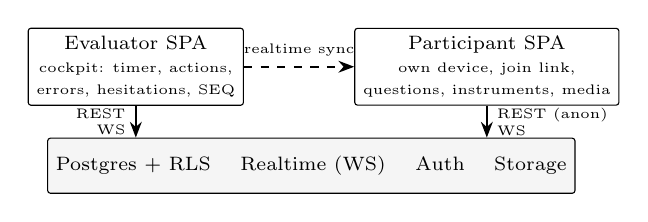
\begin{tikzpicture}[
  node distance=4mm and 6mm,
  box/.style={draw, rounded corners=1pt, align=center, font=\scriptsize,
              inner sep=3pt, minimum height=7mm},
  cloud/.style={box, fill=gray!8},
  arr/.style={-{Stealth[length=2mm]}, thick}
]
\node[box, minimum width=26mm] (eval) {Evaluator SPA\\\tiny cockpit: timer, actions,\\\tiny errors, hesitations, SEQ};
\node[box, minimum width=26mm, right=14mm of eval] (part) {Participant SPA\\\tiny own device, join link,\\\tiny questions, instruments, media};
\node[cloud, minimum width=56mm, below=9mm of $(eval)!0.5!(part)$] (supa)
  {Postgres + RLS \quad Realtime (WS) \quad Auth \quad Storage};
\draw[arr] (eval) -- node[left, font=\tiny, align=right] {REST\\WS} (eval |- supa.north);
\draw[arr] (part) -- node[right, font=\tiny, align=left] {REST (anon)\\WS} (part |- supa.north);
\draw[arr, dashed] (eval) -- node[above, font=\tiny] {realtime sync} (part);
\end{tikzpicture}
\caption{Architecture: two browser roles over a shared Postgres backend;
row-level security scopes evaluator data to accounts and participant
access to per-session join codes; realtime channels synchronize both
views.}
\label{fig:arch}
\end{figure}

\subsection{Protocol Model}
A \emph{template} is a reusable test protocol: an ordered set of
\emph{tasks}, optionally grouped, each carrying instructions and optimal
time/action baselines; a study-specific \emph{error taxonomy} (code plus
label, e.g.\ \emph{WB, wrong button}); \emph{per-task questions} of seven
types (open text, single and multiple choice, rating, audio, video,
photo); a semi-structured \emph{interview script}; and \emph{participant
fields}: extra attributes such as handedness or vision correction that
the study collects per participant. Templates also select the
post-session instruments a study administers, in any combination: the
SUS~\cite{brooke1996sus}, the unweighted (raw) NASA-TLX workload
scale~\cite{hart2006nasatlx}, and the eight-item UEQ-S user experience
questionnaire~\cite{schrepp2017ueqs}. None is mandatory, because they
answer different questions. A study of a system operated under time
pressure may need workload and not perceived usability; a comparison of
two designs' experiential appeal may need UEQ-S alone; a formative study
run mid-iteration may need no questionnaire, its evidence being the
problems observed. Opting out remains a visible decision rather than an
oversight: the protocol review of Section~\ref{sec:pedagogy} notes a template that
administers no instrument at all, with the reason a standardized scale
matters. A \emph{session} instantiates a
template for one participant and accumulates per-task results (status,
time, action count, error and hesitation logs with timestamps, SEQ),
question answers, interview answers, and the item scores of every
administered instrument.
Participants can be enrolled directly, through single-use personal links,
or through shared links that spawn one session per respondent, with
configurable collection (or omission, for anonymous participation) of
identity fields. Task presentation order is a per-session strategy chosen
at creation: the template's fixed order, an independent random shuffle,
or Latin-square rotation in which consecutive sessions rotate the
starting task so that every task occupies every position equally often
across the cohort; the strategy is recorded on the session and stated in
its report.

\subsection{Live Session and Synchronization}
During a session the evaluator's cockpit drives the protocol
(Fig.~\ref{fig:ui}). Completing a task opens the SEQ prompt and advances a
persisted task pointer; the participant's device follows that pointer and
shows the active task's instructions, so the facilitator never has to read
them aloud. When the evaluator marks a task complete, its questions unlock
on the participant's device; conversely, the evaluator's
success/partial/failure controls are \emph{disabled} while the participant
is still answering the previous task's questions, with a notification when
they finish: a two-way gate designed to keep both roles aligned without
requiring verbal coordination (Fig.~\ref{fig:seq}). Both directions of the gate are
computed from persisted state (the task pointer and the ratio of answers
to questions per completed task), not from ephemeral messages, so either
client can reload or lose connectivity mid-session and rejoin in a
consistent state. The evaluator can step back one task without destroying
recorded data, or explicitly reset a task (clearing its metrics, logs, and
answers) after confirmation. After the last task the participant answers
the interview, when the template has one, and then each instrument the
template administers, on their own device; scores are computed
automatically, and SUS scores are banded~\cite{bangor2009determining,
sauro2011practical}.

\begin{figure}[t]
\centering
\resizebox{\columnwidth}{!}{%
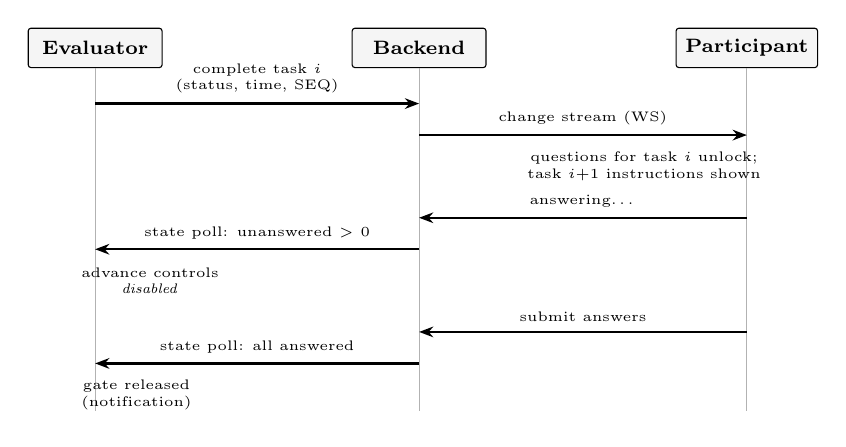
\begin{tikzpicture}[
  font=\scriptsize,
  lane/.style={draw, rounded corners=1pt, fill=gray!8, minimum width=17mm,
               minimum height=5mm, font=\scriptsize\bfseries},
  msg/.style={-{Stealth[length=1.8mm]}, thick},
  note/.style={font=\tiny, align=center}
]
\node[lane] (E) {Evaluator};
\node[lane, right=24mm of E] (DB) {Backend};
\node[lane, right=24mm of DB] (P) {Participant};
\draw[gray!60] (E.south) -- ++(0,-4.35);
\draw[gray!60] (DB.south) -- ++(0,-4.35);
\draw[gray!60] (P.south) -- ++(0,-4.35);
% task advance
\draw[msg] ($(E.south)+(0,-0.45)$) -- node[above, note]{complete task $i$\\(status, time, SEQ)} ($(DB.south)+(0,-0.45)$);
\draw[msg] ($(DB.south)+(0,-0.85)$) -- node[above, note]{change stream (WS)} ($(P.south)+(0,-0.85)$);
\node[note, anchor=east] at ($(P.south)+(0.3,-1.25)$) {questions for task $i$ unlock;\\task $i{+}1$ instructions shown};
% gate on
\draw[msg] ($(P.south)+(0,-1.9)$) -- node[above, note]{answering\ldots} ($(DB.south)+(0,-1.9)$);
\draw[msg] ($(DB.south)+(0,-2.3)$) -- node[above, note]{state poll: unanswered $>$ 0} ($(E.south)+(0,-2.3)$);
\node[note, anchor=west] at ($(E.south)+(-0.3,-2.7)$) {advance controls\\\emph{disabled}};
% gate off
\draw[msg] ($(P.south)+(0,-3.35)$) -- node[above, note]{submit answers} ($(DB.south)+(0,-3.35)$);
\draw[msg] ($(DB.south)+(0,-3.75)$) -- node[above, note]{state poll: all answered} ($(E.south)+(0,-3.75)$);
\node[note, anchor=west] at ($(E.south)+(-0.3,-4.15)$) {gate released\\(notification)};
\end{tikzpicture}%
}
\caption{Two-way gating during a moderated session. The participant
follows the evaluator over a realtime channel; the evaluator's gate is
refreshed by short-interval polling of the same persisted state, so
either client can reload mid-session and rejoin consistently.}
\label{fig:seq}
\end{figure}

\subsection{Measures}
For each task $i$ the platform records completion status
$s_i \in \{\text{success},\text{partial},\text{failure},\text{skipped}\}$,
time on task $t_i$, evaluator-counted actions $a_i$, categorized error and
hesitation events with within-task timestamps, and the SEQ rating
$q_i \in [1,7]$. Templates supply per-task baselines $t^{*}_i$ (optimal
time) and $a^{*}_i$ (optimal action count), following the
optimal-path-referenced efficiency measures recommended in the
measurement literature~\cite{albert2022measuring,sauro2016quantifying}.
Session-level indicators are the completion-status distribution, mean
time and action efficiency
$\frac{1}{|A|}\sum_{i \in A} t^{*}_i / t_i$ (and analogously for
actions), where $A$ contains only \emph{attempted} tasks with
$t_i > 0$ (skipped tasks are excluded rather than scored as zero-time
successes, an aggregation rule we adopted after observing that including
them produces unbounded efficiency values), and, when the SUS is
administered, its score with the adjective
band~\cite{brooke1996sus,bangor2009determining}. Cross-session
SUS summaries are accompanied by two-sided 95\% confidence intervals
computed with the $t$-distribution, following the small-sample
recommendation of Sauro and Lewis~\cite{sauro2016quantifying}. A
second rater can score a completed session's tasks independently; the
platform then reports Cohen's $\kappa$~\cite{cohen1960kappa} on
completion status, read against the Landis and Koch
bands~\cite{landis1977measurement}, and exact-match rate, mean absolute
difference, and Pearson correlation on action, error, hesitation, and
SEQ counts, making the reliability of evaluator-logged measures
measurable per session rather than assumed. The cockpit also records the
corrections made while logging (an undone action, error, or hesitation, a
return to the previous task, a task reset, a timer reset), which would
otherwise leave no trace, since an undo deletes what it undoes. A reset in
particular changes how a result must be read: the participant attempted the
task twice, and its recorded measures describe only the second attempt, so
the session view names it. The cockpit writes a marker when it opens, which
lets a session logged without corrections be told apart from one that was
not recorded at all. When a
template administers them, raw NASA-TLX is scored as the unweighted mean
of its six subscales~\cite{hart2006nasatlx} and UEQ-S as pragmatic,
hedonic, and overall means on the $-3$ to $+3$
scale~\cite{schrepp2017ueqs}. The participant client administers all
instruments in English or European Portuguese, the SUS items following
a validated Portuguese translation.
Distributions, efficiency ratios, and SUS scores are computed at display
time from the stored task results; per-task error, hesitation, and action
counts are persisted when the task completes, alongside the individual
timestamped log entries they summarize.

Because evaluator-counted actions are a manual measure, the platform can
optionally instrument browser-based systems under test directly: a
dependency-free script embedded in the tested system streams click,
keypress, and navigation events (element descriptors and key classes
only, never typed text) into the running session, keyed by its join code
and accepted server-side only while the session is in progress. The
evaluator cockpit shows the automatic counts beside the manual tally
during the session, the results view charts the captured event stream
over session time, and the events export as a raw table, enabling a
manual-versus-automatic count comparison as an internal validity check
on the action measure.

\begin{figure}[t]
\centering
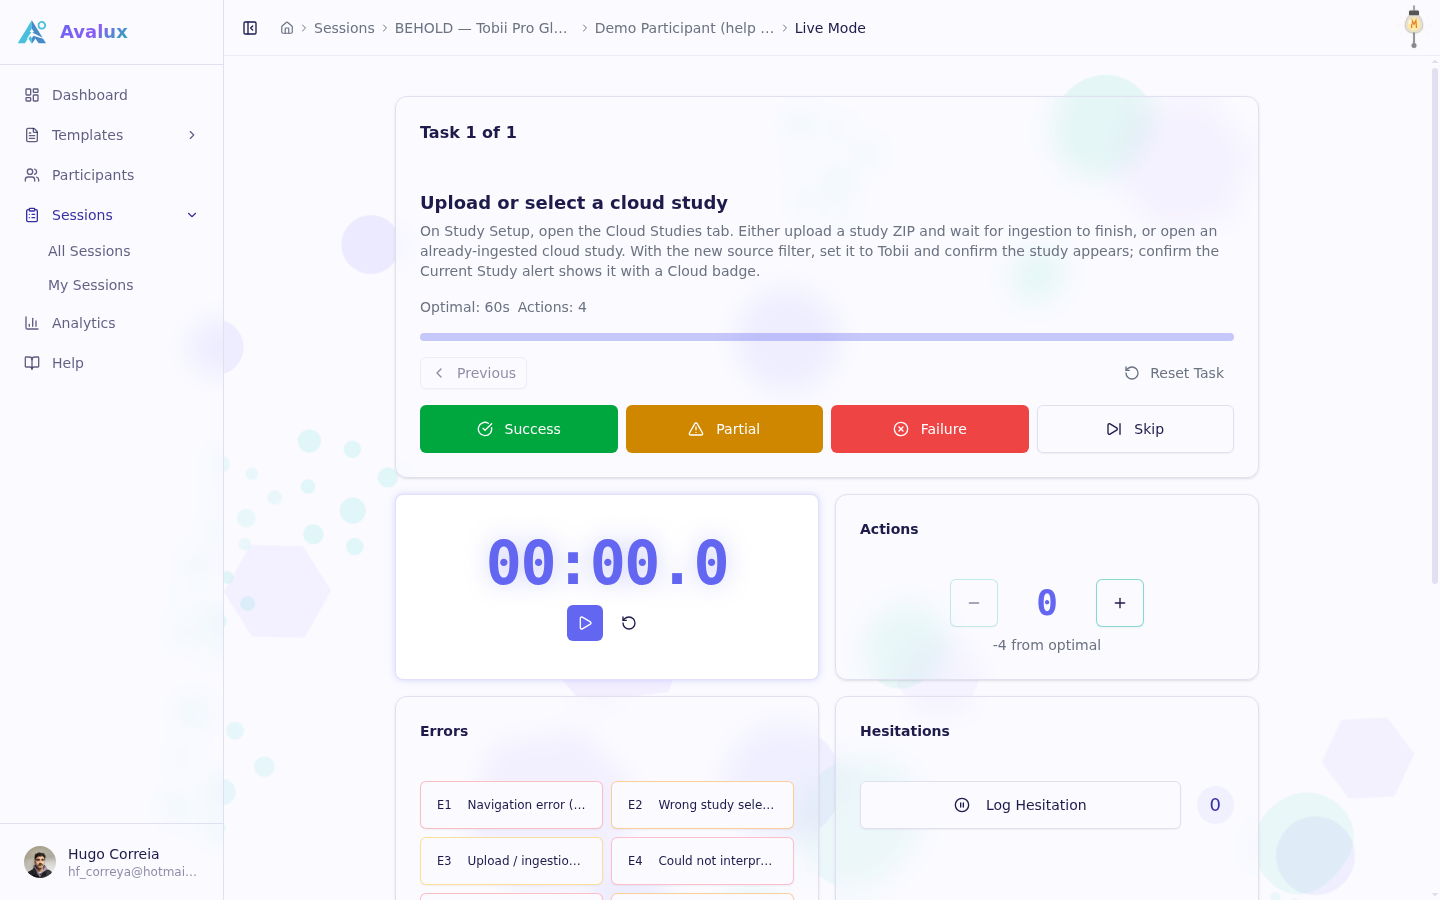
\includegraphics[width=\columnwidth]{figures/ui-live.png}
\caption{Evaluator cockpit during a live session: task navigator with
completion controls, timer, action counter, one-tap typed error logging,
and hesitation logging.}
\label{fig:ui}
\end{figure}

\subsection{Security Model}
\label{sec:security}
The platform's least conventional engineering choice is placing the whole
authorization model inside the database. Evaluator tables carry policies
of the form \texttt{user\_id = auth.uid()}; participant access is granted
to the anonymous role through policies that join the target row to a
session whose unguessable \texttt{join\_code} is non-null, so possession
of a link is the capability to act in exactly one session. Because
participants must also \emph{write} (answers, SUS items, media
references), each such table pairs a scoped \texttt{INSERT}/\texttt{UPDATE}
policy with the read policy, and mutable invitation counters are further
restricted with column-level grants so an anonymous client can increment
a response counter but not rewrite an invitation's task selection. This
model survived two studies without an application server, though it
requires discipline: one gap, a missing anonymous update policy on
invitation counters, which silently aborted link joins after the
participant row was already created, was found during operation and is
now covered by a regression migration. Participant media (photo, audio,
and video answers) lives in a private bucket and is served exclusively
through short-lived signed URLs, so a leaked link expires instead of
exposing a recording permanently; deleting a session also deletes its
stored media. Studies that must avoid personal data can disable identity
collection entirely, producing anonymous participant records that never
join the evaluator's roster, and a completed session's participant can be
anonymized retroactively (identity replaced, contact details and custom
attributes removed, demographics and metrics kept). Operational error
monitoring follows the same stance: only uncaught exceptions are
reported, tagged with opaque session identifiers, with no session
replays, no performance traces, and no request payloads.

Evaluators can optionally group into organizations; a template assigned
to an organization, with its sessions, becomes accessible to members
through additive membership policies layered over the per-user rules,
so collaboration never widens anonymous participants' access. A
restricted student role scopes selected members to individually
assigned templates, supporting classroom deployments in which each
student group runs its own project under a supervising account, and
anyone with read access to a running session can follow it on a
read-only observation view, attaching timestamped observer notes that
export alongside the session data.

\subsection{Analysis and Reporting}
Session dashboards chart completion status, time and action counts against
the template's optimal baselines, error and hesitation distributions, SEQ
per task, and a normalized per-task performance radar
(Fig.~\ref{fig:dash}); per-task event timelines plot each logged error
and hesitation at its within-task timestamp, showing \emph{when} inside a
task problems clustered; template-level analytics aggregate all completed
sessions. A one-click export renders a self-contained PDF report
(participant demographics, per-task tables, charts, timelines, logs,
interview answers, and questionnaire breakdowns with cross-session
comparison), replacing the manual assembly step that typically follows
moderated studies. For external statistical analysis, every measurement a
study produced can also be exported as raw flat tables (CSV or JSON):
sessions, task results with baselines, timestamped event logs, question
answers, and per-item questionnaire scores.

\subsection{Qualitative Coding}
Beyond the quantitative record, the platform supports a lightweight
qualitative analysis workflow directly on collected text. Each template
carries a code book: a set of short, color-coded labels with optional
definitions, authored by the evaluator. Any open-ended task answer or
post-session interview answer can then be tagged with any number of
codes from the session's results view, and a code-frequency matrix
(codes as rows, sessions as columns) aggregates tag counts at the
template level as coding proceeds. Tags are exported as their own raw
table alongside the quantitative data, with each tag row resolving the
coded answer's text, source question, and session, so downstream
analysis can move between counts and quotes. Commercial platforms
typically confine tagging to recorded video timelines in their
unmoderated products; coupling a template-scoped code book to the
structured answers of moderated sessions keeps the coding unit aligned
with the protocol itself.

\subsection{Heuristic Inspection and Synthesis}
\label{sec:inspection}
Usability testing is ordinarily preceded by inspection, in which evaluators
judge an interface against a short set of principles without
participants~\cite{nielsen1990heuristic}. Avalux supports it as the stage
before a protocol is written. A team inspects its own prototype or, before
one exists, a comparable product, against a heuristic set; Nielsen's ten
heuristics~\cite{nielsen1994enhancing} are built in, and the schema admits
sets defined by an organization. Each finding records a description and
optionally a heuristic, a location, and a severity from 0 (not a problem)
to 4 (catastrophe).

Evaluators work alone. Row-level security refuses to return another
evaluator's findings until both have submitted, and submission freezes a
pass so that it cannot be revised after reading the others; an organization
owner who is not an evaluator sees who has submitted, but no findings,
until every pass is in. The statistic that follows depends on this rule.
Hertzum and Jacobsen attribute part of the evaluator effect to vague
evaluation procedures leading to anchoring~\cite{hertzum2001evaluator}, and
an evaluator who reads a teammate's list first inflates exactly the
agreement being measured. The passes are then merged into one problem list,
and three figures describe the merge: any-two agreement, the mean over all
pairs of evaluators of the problems they share divided by the problems they
found between them, as Hertzum and Jacobsen define it; the share of
problems that only one evaluator found; and the expected number of problems
found by every possible group of $k$ evaluators, computed exactly over
subsets, with the number of evaluators the discovery model of Nielsen and
Landauer~\cite{nielsen1993mathematical} predicts for three quarters and nine
tenths of the known problems. A cohort thus derives the familiar
advice on how many evaluators to use from its own passes, rather than
receiving it.

After testing, the same list is set against what participants did. Each
predicted problem is marked as encountered, not observed, or not yet
tested, and linked to the sessions that show it; problems testing revealed
but inspection did not predict are recorded alongside. A session may serve
as evidence only for a problem of its own study, a rule enforced in the
database, and the interface does not offer pilot sessions as evidence. Two ratios
follow. Of the tested predictions, the share participants encountered is
the \emph{validity} of the inspection, and of the problems testing showed,
the share the inspection predicted is its \emph{thoroughness}, measures
defined by Sears~\cite{sears1997heuristic} and systematized by Hartson et
al., who make both relative to an \emph{actual criterion} that decides
which problems are real~\cite{hartson2001criteria}. Here that criterion is
the team's own testing, and three consequences are built in. First, no
prediction is ever recorded as a false alarm, because laboratory testing is
not an ultimate criterion: a typical test will miss some usability
problems, and its tasks are chosen by the people who designed
it~\cite{hartson2001criteria}. Second, predictions that no task exercised
are left out of both ratios rather than counted against the inspection, a
deliberate departure from the definition of validity, whose denominator is
every problem reported. Third, the reference set is what testing showed and
never the union of inspection and testing results, since a union would make
the validity of every contributing method equal to one by
construction~\cite{hartson2001criteria}.

\subsection{Design Notes}
Two design decisions proved more consequential than expected. First,
\emph{logging must not compete with observation}: every evaluator action
during a task (counting an action, categorizing an error, marking a
hesitation) is a single tap on a persistently visible control, sized to
mobile touch-target guidelines so the cockpit is operable on a tablet
held in the lap while watching the participant. Instruments that require
navigation or typing (task questions, notes) are deferred to task
boundaries. Second, \emph{the protocol is an artifact, not
configuration}: because a template fully encodes tasks, baselines,
taxonomies, and instruments, it can be reviewed before the study like a
questionnaire, reused across sessions unchanged, exported as printable
observation sheets when a study must run entirely on paper, and, as in
study~2, seeded from a written protocol document under version control.

\begin{figure}[t]
\centering
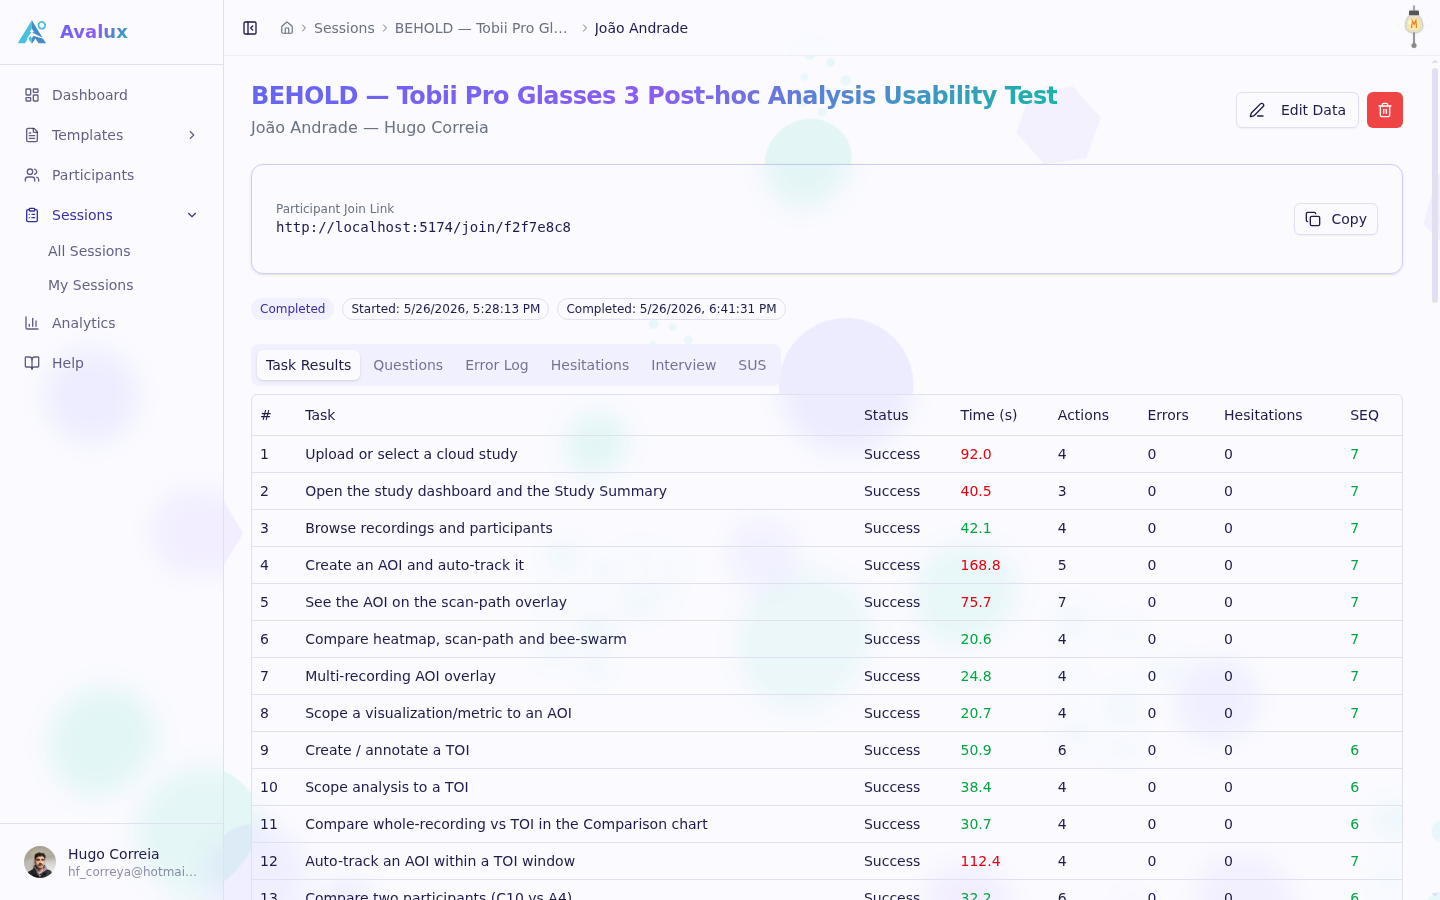
\includegraphics[width=\columnwidth]{figures/ui-session-detail.png}
\caption{Session results dashboard: per-task outcomes with time, action,
error, hesitation, and SEQ columns; charts below compare performance
against the template's optimal baselines.}
\label{fig:dash}
\end{figure}

\subsection{Model Assistance, and Its Limits}
\label{sec:assistance}
Two steps in the workflow are slow in a way that is clerical rather than
intellectual. Merging a dozen evaluators' findings into one problem list is
the longest manual step of an inspection, and after a set of sessions the same
problem appears in several of them described differently each time. Both are
the same operation: deciding which descriptions refer to one underlying
problem. A language model can propose that mapping. Whether it should is a
pedagogical question before it is a technical one, because the operation it
performs is precisely the one the exercise is meant to teach.

The platform answers that with four constraints, each enforced in the database
rather than in the interface, so that no client and no future feature can
bypass them. First, an organization opts in, and the default is off: text
leaves the system, so the decision belongs to whoever is accountable for the
data rather than to a student mid-assignment. Second, and most important for
the teaching argument, a suggestion cannot be obtained before the team has
done the work itself. For an inspection, the row-level policy that releases
other evaluators' findings only after every pass is submitted already gates it,
so no student can read a proposed problem list before writing their own
findings; for a study summary, the request is refused until the team has
entered at least one problem of its own. Assistance is available for what a
team might have missed, never as a substitute for looking. Third, nothing is
applied automatically. A proposal is a stored record that a person accepts or
dismisses, and accepting it writes the same rows the person would have written
by hand, marked \emph{assisted}, so a report, the data export and the
classroom study can separate assisted work from unassisted. Fourth, the
model's answer is treated as untrusted input: a validator drops finding
identifiers that do not exist, refuses to place one finding in two problems,
rejects heuristic codes outside the inspection's own set and severities off the
scale, and reports what it discarded, so a team is told when a proposal
referred to three findings that were never written.

What may be sent is decided in two tiers. Text the students wrote, their
findings, observer notes and the moderator's recorded corrections, rides on the
organization's decision. Text a participant wrote is different in kind: it was
given under a consent text that almost certainly said nothing about a language
model. Its release is therefore decided per study, defaults to off, and is
refused until the consent text contains a specific clause that the platform
supplies and then checks for. Eligibility is then a timestamp comparison rather
than a promise in the interface. Enabling the option records the instant it was
enabled, and a session qualifies only if its own recorded consent is at or
after that instant. The consequence is deliberate and, in our experience of
explaining it, initially surprising: a study whose sessions have already run can
never have their answers included, whatever is set afterwards, and switching
the setting off and on does not re-date it in either direction. A class that
wants this must decide before recruiting, which is the same order in which
consent itself has to be obtained. Session identifiers, participant names and
dates are never sent; sessions are numbered.

Deployment is provider-agnostic by construction. The feature runs as a server
function configured by three environment variables, an endpoint, a model and a
key, so a department that objects to student text reaching a third party can
point it at a model on its own infrastructure without a code change, and a
deployment that sets no key answers that no model is configured while
everything else continues to work. We report this as a design, not as a result:
the quality of the groupings a model proposes, and whether assisted teams
learn more or less than unassisted ones, are exactly what the \emph{assisted}
marking exists to let the classroom study measure, and neither question is
answered here.

\subsection{What Integration Buys}
\label{sec:integration}
Each instrument described above exists in some form in an ad-hoc toolchain: a
stopwatch times a task, a spreadsheet holds counts, a form collects a
questionnaire. The claim for a single platform is not that any one of them is
novel, but that four things follow from their sharing one record, and each can
be checked against the implementation rather than taken on faith.

\emph{A measurement is recorded once.} The evaluator logs a count, an error,
or a rating at the moment of observation, and the session dashboard, the
cross-session analytics, the PDF report, and the raw export are all reads of
that same row. Nothing is transcribed between tools, so the failure mode of the
ad-hoc pipeline, a number that changes or disappears between the observation
sheet and the report, has nowhere to occur. The report is rendered rather than
assembled.

\emph{Definitions travel with the data.} Success criteria, optimal-path
baselines, the error taxonomy, and the choice of instruments live in the
template, so every session of a study is scored against the same definitions,
and every team that shares a template in a course uses the same ones. When
those definitions live in a document beside a spreadsheet, drift between
sessions is possible and invisible; here a change to them is a change to the
protocol, which returns it to draft when it is under review.

\emph{Evidence stays attached to claims.} A merged inspection problem can
become a task, which records the problem it came from; the task produces
per-task results in each session; a problem is marked encountered only with the
sessions that show it; a report states $\kappa$ and an interval from the rows
they summarize. Each link is a stored reference, so ``why is this task here''
and ``what supports this claim'' are questions the platform answers by
navigation. In a set of separate documents those links exist only in the
author's memory of assembling them.

\emph{Coordination disappears from the session.} The gating protocol and the
participant's own device remove the verbal exchange that otherwise punctuates
a moderated session, and the evaluator never leaves the cockpit to hand over a
questionnaire.

Integration also costs. A protocol must be encoded before a study runs, which
front-loads effort a paper observation sheet never demands; a measure the
model does not support cannot simply be written in a spare column; and a single
system is a single point of failure, mitigated here only by the platform being
open, self-hostable, and able to export every row it holds. None of this is a
measured productivity claim: that the integrated pipeline is faster or more
complete than the ad-hoc one is what the counterbalanced evaluator study of
Section~\ref{sec:future} is designed to test, and until it runs the argument
above is structural, not empirical.

\subsection{Pedagogical Design}
\label{sec:pedagogy}
Avalux is also deployed in an undergraduate HCI course, where student
teams each run a moderated study of a system they are
designing~\cite{churchill2013teaching}, a setting in which, as Related Work
notes, tools built for the purpose are rare and rarely
evaluated~\cite{lima2019tools}. What novices actually find hard has been
characterized empirically rather than assumed: Oleson et al.\ identify
eighteen types of learning difficulty in HCI design education, among them
why an activity is done this way (\textsc{why}), how to perform a method
(\textsc{how}), how to interpret feedback (\textsc{synth}), how to avoid
biasing one's own design (\textsc{bias}), when to move to the next stage
(\textsc{stage}), and a tendency to rush to implementation and discount
design work (\textsc{rush})~\cite{oleson2020difficulties}.
Table~\ref{tab:pedagogy} names, for each objective, the difficulty it
addresses, so the alignment rests on reported difficulty rather than on our
own assumption about what is hard, and states the constructive
alignment~\cite{biggs1996alignment} between each objective, what the
platform offers toward it, and the evidence that would show it met; that
third column is also the rubric of the classroom study in
Section~\ref{sec:future}.

A tool that makes an expert faster does not thereby make a novice better;
the education literature separates \emph{productivity tools} from
\emph{mindtools}, which engage the learner in thinking about the
domain~\cite{jonassen2000mindtools}. Our claim is of the second kind, and
the clearest way to see the difference from the traditional stopwatch and
spreadsheet is in what the features cost. A productivity tool removes
steps. Several of Avalux's add them: a second rater scores a session that
is already scored, evaluators inspect alone before merging, each prediction
is checked against the sessions, and whoever took part in a session is
asked to reflect on it. Every added step produces evidence about the method
rather than about the design under test, and each turns a property that a
course would ordinarily assert in a lecture into a figure computed from the
team's own work: that careful evaluators disagree (Cohen's $\kappa$ on
completion, any-two agreement across inspection passes), that one
evaluator is not enough (the discovery curve of the team's own passes),
that inspection and testing find different problems (the two ratios of
Section~\ref{sec:inspection}), and that five participants license only a
wide interval (confidence intervals beside SUS). The traditional approach
can state each of these, but it cannot hand a team the figure for its own
study without an analysis nobody performs by hand, and an instructor who
receives only a final report cannot tell whether moderation was biased,
whether two observers would have logged the same errors, or whether the
sample supports the conclusion. That rests on the cognitive-apprenticeship
observation~\cite{collins1989cognitive} that expert practice is invisible
to novices until made visible, scaffolded, and reflected on, and the
features below are grouped accordingly.

\emph{Made visible.} The disagreement co-rating reveals is not a student
failing. Reviewing eleven studies of cognitive walkthrough, heuristic
evaluation, and thinking-aloud, Hertzum and Jacobsen report that average
agreement between any two evaluators of the same system ranges from 5\% to
65\%, and that the effect holds for experienced and novice evaluators alike
and for severity ratings as well as problem
detection~\cite{hertzum2001evaluator}. They attribute it to vague goal
analyses, vague evaluation procedures, and vague problem criteria:
precisely the three things a protocol template is forced to make explicit
before a session runs. Measuring $\kappa$, or the agreement of inspection
passes, therefore does more than grade a pair of students; it exposes a
property of the method itself.

\emph{Scaffolded.} The protocol review gives feedback, checking a template
without blocking against common novice mistakes (tasks that name interface
labels and so lead the participant, tasks without a success criterion or
optimal path, no practice task, no error taxonomy, no post-session
instrument), each with a rationale linked to the tutorial. Its review
appears only once a design is saved, not while it is typed: students value
procedural scaffolding but distrust it when it pre-empts their own
judgment~\cite{aziz2026genai}, and a deterministic check carries none of
the sycophancy they report in generative facilitators. Existing support for
student studies addresses planning: a toolkit for method selection, power,
and counterbalancing~\cite{schwind2023toolkit}, and a widely used plan
template whose assessment turns on an instructor gate before any session
may run~\cite{rose2016plan}. Avalux begins where they stop, at the session
itself. Its own gate, enabled per template at an organization's discretion,
is deliberately narrower than that template's. Schwind et al.\ warn that
close supervision calls into question the independence of a student's
research work~\cite{schwind2023toolkit}, so approval gates
\emph{recruiting} and not \emph{rehearsal}: a team may run its protocol
before approval, and those sessions are recorded as pilots and excluded
from the template's aggregates. The instructor thus reviews with the
protocol review's findings and the team's own pilot data in hand, without
having authored the protocol. Every decision is kept, together with the
protocol exactly as it was submitted, so two consecutive submissions are
the before and after of one revision and the mistakes that survive a
review can be counted rather than recalled.

\emph{Reflected on.} After every completed session, each person who took
part answers three fixed questions: what they did not expect, what they
would change in the protocol, and what they did that may have led the
participant. The questions sit beside what the session recorded (tasks
failed, reset, or taking twice the expected time, hesitations, a high ease
rating on a task that went badly, and notes from anyone observing), so the
answer is drawn from evidence rather than from memory. A reflection stays
private until submitted and cannot be revised afterwards, and a teammate's
becomes readable only once one's own is submitted: the same rule as for
inspection passes, since an account written after reading another's is
anchored to it.

For the instructor, a class view gives one row per project, with what
needs attention first and, as columns, the evidence of
Table~\ref{tab:pedagogy} wherever the platform records it. It reads
through the same row-level security as every other view, so an inspection
still collecting passes contributes its progress and none of its findings.
It deliberately omits the two outcomes the platform cannot observe, whether
a report states its uncertainty and whether a warning was resolved with a
written justification, rather than display a figure for them.

These are design arguments, not yet results. The platform acts on
difficulties of method execution and interpretation, not on difficulties
of design itself (\textsc{what}, \textsc{adapt}, \textsc{divrs}) or of
teamwork, scope, and stakeholders, and an added step does not guarantee
that it is taken seriously. Whether the evidence these features produce
changes what students understand is the question of the classroom study in
Section~\ref{sec:future}.

\begin{table}[t]
\caption{Constructive alignment: each learning objective, what the
platform offers toward it, and the evidence that it was met. Small capitals
name the learning difficulty of Oleson et al.~\cite{oleson2020difficulties}
that the objective addresses.}
\label{tab:pedagogy}
\centering
\footnotesize
\setlength{\tabcolsep}{4pt}
\begin{tabular}{@{}>{\raggedright\arraybackslash}p{0.30\columnwidth}>{\raggedright\arraybackslash}p{0.30\columnwidth}>{\raggedright\arraybackslash}p{0.31\columnwidth}@{}}
\toprule
Learning objective & What Avalux offers & Evidence of outcome \\
\midrule
Inspect before testing, with several evaluators (\textsc{how}) & Independent heuristic passes, hidden from one another until submitted & Passes submitted independently; any-two agreement reported \\
Say why a method step matters (\textsc{why}) & Protocol review: every check carries a rationale linked to the tutorial & Warnings resolved with a written justification \\
Write tasks as goals, not procedures (\textsc{bias}) & Protocol review, leading-task check & Warnings resolved before the first session \\
Fix criteria and baselines before running (\textsc{how}) & Success criterion and optimal path per task & Both present on every measured task \\
Control order effects (\textsc{how}) & Order strategy per session, with explainer & Strategy chosen and justified in the report \\
Treat ``error'' as a judgement (\textsc{synth}) & Co-rating, Cohen's $\kappa$ & $\kappa$ reported; disagreements reconciled \\
Report uncertainty with small $n$ (\textsc{synth}) & SUS with 95\% CI & An interval beside every score \\
Moderate without leading (\textsc{bias}) & Observation view, timestamped notes & Peer notes on hints and interventions \\
Analyse qualitatively as a procedure (\textsc{how}) & Code book, frequency matrix & Codes defined before tagging; matrix reported \\
Know when a protocol is ready to run (\textsc{stage}, \textsc{rush}) & Optional instructor gate; unapproved runs recorded as pilots; every decision kept & Approval before the first recruited participant; revisions address the review \\
Test predictions against observation (\textsc{synth}) & Predicted problems marked encountered or not observed, linked to sessions & Validity and thoroughness reported, untested predictions stated \\
Reflect on a session from its evidence (\textsc{synth}, \textsc{bias}) & Reflection prompt beside recorded failures, resets, and observer notes & A submitted reflection for every session \\
Handle participant data ethically & Retroactive anonymization, private media, per-template consent recorded at join & Anonymized export; a consent record for every participant \\
\bottomrule
\end{tabular}
\end{table}

\section{Case Studies}
Two studies were run end to end on the platform. Both used in-person,
co-located moderated sessions in which the participant handled the system
under test while the evaluator logged performance in Avalux. Study~1 used
the evaluator client alone; study~2 additionally used the participant's
own device for questions, interview, and SUS via join links, so the
synchronization and gating mechanism of
Section~III-C was exercised only in study~2's co-located
sessions; its validation with a non-co-located moderator remains future
work. Participants in both studies were volunteers recruited from the
authors' university environment, were informed about the study's purpose
and the data collected (including, in study~2, browser-captured
screenshots and recordings), and consented to participate.
In line with the responsible institution's guidelines, this
minimal-risk usability evaluation with adult volunteers did not require
formal ethics review. Participants received no compensation, gave
informed consent before their session after being briefed on the
study's goals, the tasks, and the data collected (including, in
study~2, screen and audio recordings), and could withdraw at any time
without consequence. Collected data are stored pseudonymously, and
identifying fields can be removed retroactively through the platform's
anonymization mechanism.

\subsection{Study 1: Household Touch-Panel Controller}
Four participants (ages 20--23, two female, three of low and one of high
self-rated technical proficiency) attempted 14 tasks, seven simple
(e.g.\ wake the panel, read the time, adjust temperature) and seven
complex (e.g.\ set the clock, change language, recover from an error
state), on a commercial water-heater touch panel. Sessions averaged
15~minutes. Aggregate completion across the $4\times14$ task attempts was
approximately 70\% success, 20\% partial, and 11\% failure (percentages
independently rounded). SUS scores were 25.0, 40.0, 17.5, and 30.0 (mean 28.1,
95\% CI $[13.1, 43.1]$, ``Poor''~\cite{bangor2009determining}; even the
interval's optimistic bound sits far below the benchmark mean of
68~\cite{sauro2011practical}); notably the high-proficiency participant
produced the \emph{lowest} score, indicating problems not attributable to
inexperience. Task-level metrics located the failures precisely
(Table~\ref{tab:bosch}): the undiscoverable wake-up gesture (SEQ 1.8, all
participants struggled), error recovery without any error feedback (SEQ
2.5, participants resorted to power cycling), and clock adjustment
(43.6~s and 10 actions against an optimal 8). Participants' reports of
buttons changing function across screens figured among the study's
principal design recommendations, alongside a persistently visible entry
point to settings and explicit error feedback.

\begin{table}[t]
\caption{Study 1: selected task-level results ($N{=}4$).}
\label{tab:bosch}
\centering
\footnotesize
\setlength{\tabcolsep}{4pt}
\begin{tabular}{@{}lccl@{}}
\toprule
Task & Mean SEQ & Mean time (s) & Note\\
\midrule
Wake up panel & 1.8 & -- & all struggled\\
Recover from error & 2.5 & -- & no error feedback\\
Set clock to 08:30 & -- & 43.6 & 10 actions vs.\ 8 optimal\\
Read current time & 7.0 & 2.7 & 100\% success\\
\bottomrule
\end{tabular}
\end{table}

\subsection{Study 2: Eye-Tracking Analysis Dashboard}
The second study evaluated BEHOLD, a post-hoc analysis dashboard for
Tobii Pro Glasses~3 recordings, with two participants (ages 22--23,
students, low technical proficiency). The protocol exercised the
platform's richer features: 21 tasks in eight groups following the
analyst's journey (Table~\ref{tab:behold}), of which each session ran
20, a 19-item error taxonomy, media question types (screenshots, screen
recordings, audio narration), and custom participant fields (handedness,
vision correction, device, location).

\begin{table}[t]
\caption{Study 2: protocol structure (task groups and per-task
question instruments).}
\label{tab:behold}
\centering
\footnotesize
\begin{tabular}{@{}lcl@{}}
\toprule
Task group & Tasks & Question instruments\\
\midrule
Study ingestion & 2 & choice, open, rating, photo\\
Data browsing & 2 & choice, open, rating\\
Areas of interest (AOI) & 4 & choice, rating, open, video, photo\\
Times of interest (TOI) & 4 & choice, rating, open, video, photo\\
Visualizations & 1 & choice, photo\\
Participant comparison & 2 & choice, open, rating, photo\\
Metrics explorer & 5 & choice, rating, open, audio\\
Export & 1 & choice, rating, audio\\
\bottomrule
\end{tabular}
\end{table}

Task success was near-universal, with one consistent exception: the
fixation-metric configuration task in the metrics explorer failed for
both participants, isolating the dashboard's least intuitive workflow;
every other task was completed successfully by both participants (one
task was skipped in one session). Both participants scored the system at
SUS 80 (``Good'', approaching
``Excellent''~\cite{bangor2009determining}). Open answers
converged on three concrete defects (an auto-track feature hidden in an
overflow menu, participant IDs shown instead of names in comparisons, and
truncated axis labels), each traceable to a specific task's logs and
answers in the report.

\subsection{Cross-Study Reading}
Fig.~\ref{fig:sus} contrasts the per-participant SUS scores of both
studies against the industry benchmark. The two cohorts are comparable
(young adults in their early twenties, predominantly low technical
proficiency), yet the platform separates the two designs by more than
fifty SUS points with non-overlapping ranges, and its task-level
instruments explain \emph{where} each design earns its score. We take
this as evidence that an integrated moderated pipeline can deliver both
the discriminative summary metrics and the diagnostic detail that
typically require separate tools.

Operationally, a single evaluator ran every session in both studies. The
protocol-as-template design meant the second study's considerably richer
instrumentation (19 error codes, media questions, custom participant
attributes) cost setup effort once rather than per session, and both
study reports, including all charts and per-task appendices, were
generated without manual assembly. Running real studies also stress-tested
the platform itself: study operation exposed a row-level-security gap in
the anonymous invitation-counter update (Section~\ref{sec:security}) and showed that
evaluators under load can leave action counters untracked, both of which
fed fixes and roadmap items back into the platform.

\begin{figure}[t]
\centering
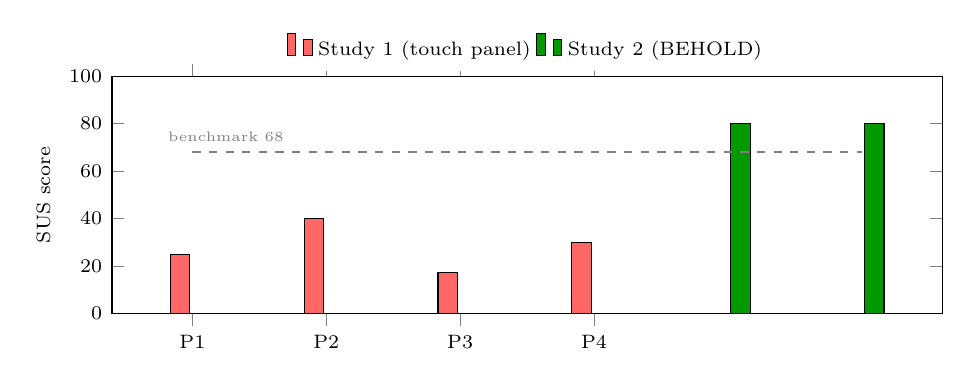
\begin{tikzpicture}
\begin{axis}[
  width=\columnwidth, height=4.6cm,
  ybar, bar width=7pt,
  ymin=0, ymax=100,
  ylabel={SUS score}, ylabel near ticks,
  symbolic x coords={S1-P1,S1-P2,S1-P3,S1-P4,S2-P1,S2-P2},
  xtick=data,
  xticklabels={P1,P2,P3,P4,P1,P2},
  enlarge x limits=0.12,
  legend style={font=\scriptsize, at={(0.5,1.02)}, anchor=south,
                legend columns=-1, draw=none},
  tick label style={font=\scriptsize},
  label style={font=\scriptsize},
]
\addplot[ybar, fill=red!60]
  coordinates {(S1-P1,25) (S1-P2,40) (S1-P3,17.5) (S1-P4,30)};
\addplot[ybar, fill=green!60!black]
  coordinates {(S2-P1,80) (S2-P2,80)};
\draw[dashed, thick, gray]
  (axis cs:S1-P1,68) -- (axis cs:S2-P2,68)
  node[pos=0.05, above, font=\tiny, gray] {benchmark 68};
\legend{Study 1 (touch panel), Study 2 (BEHOLD)}
\end{axis}
\end{tikzpicture}
\caption{Per-participant SUS scores in both case studies against the
industry benchmark mean of 68~\cite{sauro2011practical}. Participant
indices are per study; the two cohorts are unrelated.}
\label{fig:sus}
\end{figure}

\section{Discussion and Limitations}
\subsection*{Construct validity}
Action and error counts are logged by the evaluator rather than
instrumented automatically; this keeps the platform applicable to physical
devices (study~1 evaluated hardware no browser can instrument) at the cost
of observer load and potential undercounting during fast interaction
bursts, and error categorization is single-observer unless a session
is co-rated; the co-rating instrument measures agreement per session,
but a study-level reliability figure for live logging has not yet been
established. The corrections the cockpit now records give each session a
direct indicator of that load, although the case-study sessions predate
the feature and so have none. The synthesis ratios inherit the
limits of their actual criterion: a handful of sessions, on tasks the team
chose, is evidence of which predictions were encountered, not proof of
which were wrong. SEQ and SUS are self-report instruments with
known ceiling effects. The optimal-path baselines that anchor the
efficiency measures are themselves author-defined and inherit the
protocol designer's assumptions. The protocol review can be satisfied
without being understood: a student may clear its warnings
mechanically, the hazard Schwind et al.\ note for planning
toolkits~\cite{schwind2023toolkit}, which is why the classroom study
scores understanding and not only artifacts.

\subsection*{Internal validity}
Both studies were run by a single evaluator who is also the platform's
author; observer bias in logging and status judgments cannot be excluded.
The two case-study cohorts, while demographically similar, attempted
different systems with different protocols, so the cross-study SUS
contrast (Fig.~\ref{fig:sus}) should be read as discriminative range, not
as a controlled comparison.

\subsection*{External validity}
The samples (four participants in study~1, two in study~2) are in line
with problem-discovery practice
\cite{virzi1992refining,nielsen1993mathematical} but far too small for
statistical generalization of the metric values (study~2's two
participants in particular make its aggregate figures illustrative
only), and both cohorts were young adults in their early twenties. More importantly for a tool paper, we have not yet
run a controlled comparison of evaluator effort and data quality against
an ad-hoc toolchain or a commercial moderated platform; the case studies
demonstrate feasibility and output quality, not superiority; that
comparison is the designed next study (Section~\ref{sec:future}). Named in
the vocabulary of toolkit research, the two case studies are a
\emph{demonstration}: the most common evaluation strategy in toolkit papers
and the weakest on its own, since it establishes that something can be
built rather than that it is worth building~\cite{ledo2018evaluation}. The
evaluator and classroom studies of Section~\ref{sec:future} are
\emph{usage} studies. The two remaining strategies of that taxonomy,
technical performance and a heuristic analysis of the toolkit's own design,
are not yet attempted.

\subsection*{Threats to the pedagogical claim}
The argument of Section~\ref{sec:pedagogy} has threats of its own, distinct
from those of the case studies, and the classroom study is designed around
them. The platform keeps inspection passes and reflections apart, but
students who share findings in a chat are beyond its reach; the agreement of
a team's passes detects only the gross case, since agreement far above the
published range suggests the passes were not independent. The class view
shows which evidence each team has produced, which invites filling a column
without the understanding it stands for, so the study's outcomes are
understanding items and blind grading, never the columns themselves.
Instructors read submitted reflections, which may lead students to write for
the reader, so grades must not depend on what a reflection admits. Because
several features add work by design, effort differs between cohorts more
than it would for a tool that only saves time. A new tool also carries a
novelty effect that a familiar toolchain does not. The model assistance of
Section~\ref{sec:assistance} is the sharpest threat of all, since it can
perform the very operation the exercise teaches. The design answers it by
ordering rather than by prohibition, releasing a proposal only after a team has
produced its own work, and by recording which problems were accepted from a
proposal, so that a cohort using assistance can be compared with one that does
not instead of the question being assumed away. Whether that ordering is enough
is an empirical question the classroom study is designed to answer and this
paper does not. Finally, students are a captive population: taking part in the
study must be separable from the assignment, and grading should involve someone
independent of the tool's development.

\subsection*{Security surface}
The anonymous-participant model trades open link joins for RLS
policies that must admit exactly the rows a code-holder is entitled
to. An audit after the case studies found that the original
participant-flow policies tested whether a row was the \emph{kind} a
participant may see, not whether the caller held its code, which for
the anonymous role is equivalent to no policy: participant records,
answers, and live invitation codes were readable without
authenticating. The policies were rewritten to compare each row against
the code carried in the request, verified by an automated probe,
shipped with the repository, that reads every participant-facing table
as an anonymous client and fails on any row returned. The gap survived
two studies and a fix to a neighbouring policy; a policy set is now
treated as a tested artifact, not configuration.

Because the participant client is an ordinary web page, the same
protocol runs in a lab (as in both case studies), over a video call
with the join link shared in chat, or asynchronously through shared
links, though the evaluator-logged instruments apply only in the
moderated modes. Synchronous remote moderation approaches lab
quality in prior comparisons~\cite{andreasen2007remote,
brush2004comparison}; verifying that the gating protocol preserves that
equivalence with a remote moderator is a natural next experiment. The
participant-own-device model also inherits the device diversity of
field settings~\cite{kaikkonen2005usability}: the mobile-first client
followed directly from pilot participants joining on their phones.

\section{Conclusion and Future Work}
\label{sec:future}
Avalux integrates protocol definition, live moderated logging,
participant-side questioning on the participant's own device, standardized
instruments, analytics, and reporting into one open platform, and carried
two complete usability studies whose results discriminated sharply between
a poorly and a well-received design. For teaching it adds a stage before
testing and a closing one after it, independent inspection and its
comparison with what participants encountered, and between them features
chosen for the evidence they produce about the method rather than the
effort they save.

Future work proceeds on two tracks. The \emph{evaluation} track validates
the tool itself: a counterbalanced evaluator study against a
stopwatch-and-spreadsheet baseline (setup time, logging completeness,
report latency, SUS and workload on the toolchain), an inter-rater
reliability study of the live-logging instrument, and a
manual-versus-automatic action-count comparison using the
instrumentation events of Section~III to bound manual logging error.
The pedagogical framing of Section~\ref{sec:pedagogy} adds a classroom study: two
cohorts of one HCI course, using Avalux and the
stopwatch-and-spreadsheet toolchain respectively, compared on
protocol quality scored against the evidence column of
Table~\ref{tab:pedagogy}, inter-rater agreement between team
members on a shared recorded session, the proportion of reports
stating uncertainty with their estimates, and a pre/post test of
methodological understanding. That test asks, among other things, whether
students who saw their own evaluators' agreement understand why one
evaluator is not enough, and whether those who compared predictions with
testing stop reading an unobserved prediction as a false alarm; coded
reflections show whether one written beside the recorded evidence names the
moderator's own interventions more often than one written from memory; and
the protocol review, run over each kept submission, shows which mistakes
persist after feedback; it is the kind of rigorous evaluation the mapping
of HCI teaching found largely absent~\cite{lima2019tools}. The platform
now records much of what that study needs rather than leaving it to be
reconstructed: the agreement of each team's inspection passes, the ratios
of predicted to encountered problems, every protocol submission with the
reviewer's decision, from which the mistakes that persist across revisions
can be counted, a reflection for each session, and the corrections made
while logging each one, which the reliability study can set against
co-rater disagreement. The remaining gaps are narrower: instructor feedback
on an individual session rather than on a protocol, comparison of one
protocol across design iterations, a record of the consent text each
participant agreed to rather than only the moment of agreement, and
evidence images on inspection findings, withheld until they can be stored
under the same isolation rule as the findings themselves.
The \emph{platform} track continues with a more flexible task model;
the additions described in Section~III beyond the two studies' original
scope were themselves motivated by those studies and shipped since
they concluded.

\section*{Availability}
The platform is deployed at \url{https://avalux.pt}. Its source (the
application, 60 SQL migrations, the seeded protocol of study~2, the
tutorial, and the report generator) is available under the MIT license
at \url{https://github.com/hugocorreia15/usertesting}. Anonymized
session data from the case studies is available on request within the
limits of the participants' consent.

\balance
\bibliographystyle{IEEEtran}
\bibliography{refs}

\end{document}
